\subsection{Descripci\'on del problema}

Se nos pide resolver el problema de obtener un orden de fabricaci\'on de joyas tal que se minimice la p\'erdida de dinero. Para lograr esto, se sabe que cada joya $j_{i}$ posee un tiempo de fabricaci\'on $t_{i}$ y un valor de devaluaci\'on diario $d_{i}$. \\

Para calcular la p\'erdida dado un orden de fabricaci\'on, se debe calcular la siguiente f\'ormula:

$\sum\limits_{i=0}^n d_{i}*dia\_finalizacion\_joya_{i}$

Donde $n$ es la cantidad de joyas menos uno, y $dia\_finalizacion\_joya_{i}$ es el dia global en el que se termina de fabricar la joya.\\

El caso trivial ser\'ia una lista de joyas con todos los valores de devaluaci\'on diaria y tiempo de fabricaci\'on iguales, cualquier permutaci\'on de estas joyas sirve como soluci\'on optima. \\ 

Observemos algunos ejemplos mas interesantes: \\

Ejemplo 1) Dadas las joyas $j_{0}$, $j_{1}$ y $j_{2}$ con tiempos de fabricaci\'on 3, 5 y 8, y valor de devaluaci\'on 10, 30 y 15 respectivamente, la soluci\'on \'optima ser\'ia el siguiente orden de fabricaci\'on:

\begin{figure}[h]
\begin{center}
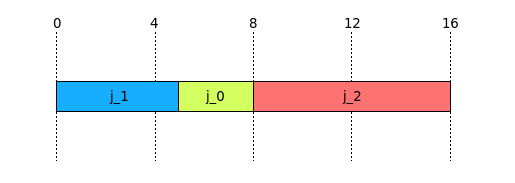
\includegraphics[scale=0.7]{./img/ej2_chart1.png}
\caption{Distribuci\'on de las joyas a fabricar}
\end{center}
\end{figure}

Esta disposici\'on se calcula con la siguiente formula:

$d_{0}*8 + d_{1}*5 + d_{2}*16 = 470$ \\

Se puede comprobar calculando la misma formula para todas las permutaciones posibles del problema que \'esta es la \'optima: \\

$d_{0}*8 + d_{1}*5 + d_{2}*16 = 470$ \\
$d_{0}*16 + d_{1}*5 + d_{2}*13 +  = 505$ \\
$d_{0}*3 + d_{1}*8 + d_{2}*16 = 510$ \\
$d_{0}*16 + d_{1}*13 + d_{2}*8 = 670$ \\
$d_{0}*3 + d_{1}*16 + d_{2}*11 = 675$ \\
$d_{0}*11 + d_{1}*16 + d_{2}*8 = 710$ \\

Ejemplo 2) Tambien puede suceder que haya mas de una soluci\'on \'optima, osea, varias permutaciones dan el valor de perdida menor. Supongamos un listado de joyas con tiempos de fabricaci\'on 5, 2 y 10 y devaluaci\'on diaria 10 40 y 20. \\

Realicemos el mismo calculo que para el ejemplo anterior y comprobemos que tiene 2 soluciones \'optimas:

$d_{0}*7 + d_{1}*2 + d_{2}*17 = 490$ \\
$d_{0}*17 + d_{1}*2 + d_{2}*12 +  = 490$ \\
$d_{0}*5 + d_{1}*7 + d_{2}*17 = 670$ \\
$d_{0}*5 + d_{1}*17 + d_{2}*15 = 1030$ \\
$d_{0}*15 + d_{1}*17 + d_{2}*10 = 1030$ \\
$d_{0}*17 + d_{1}*12 + d_{2}*10 = 850$ \\

\subsection{Resoluci\'on}

Para resolver el problema se decidio elegir algun tipo de medida de $peso$ para poder clasificar las joyas, donde $peso$ refiere especificamente a la siguiente ecuaci\'on: \\

$peso\_j_{i} = \frac{d_{i}}{t_{i}}$

Esta f\'ormula entrega una relacion entre ambas variables, luego el algoritmo procede a ordenar la fabricaci\'on de las joyas por estas relaciones de mayor a menor. \\

Una descripci\'on del algoritmo en pseudo codigo:

\begin{itemize}
\item Para cada joya, calcular la relacion devaluacion sobre tiempo de la joya
\item Ordenar las joyas segun su costo por dia
\end{itemize}

\subsection{Demostraci\'on de la resoluci\'on}

Para poder demostrar que el algoritmo funciona, recordemos como se expresaban las p\'erdidas segun la distrubuci\'on de las joyas:

$P = \sum\limits_{i=1}^n (d_{i}*( \sum\limits_{k=1}^i t_k ))$

Donde cada $d_i$ corresponde a la devaluaci\'on de la joya elegida a ocupar la posici\'on $i$ \\

La hip\'otesis que decidimos utilizar para garantizar que esa f\'ormula da un P \'optimo es:

$ \frac{d_{i}}{t_{i}} \geq \frac{d_{i+1}}{t_{i+1}} \Longleftrightarrow d_i*t_{i+1} \geq d_{i+1}*t_i $

Intentemos ver que ocurre para algunos casos:

\subsubsection*{Caso dos joyas}

Nuestra hip\'otesis es:

$d_1*t_2 \geq d_2*t_1$ \\

Veamos si podemos decidir el orden \'optimo para este caso:

$d_1*t_1 + d_2*(t_1 + t_2) \leq d_2*t_2 + d_1*(t_1 + t_2) \Longleftrightarrow $ (Distributiva)

$d_1*t_1 + d_2*t_1 + d_2*t_2 \leq  d_2*t_2 + d_1*t_1 + d_1*t_2 \Longleftrightarrow$ (Simplifico terminos)

$d_2*t_1 \leq d_1*t_2$

Si se cumple nuestra hip\'otesis podemos decidir que el orden propuesto era el \'optimo, si no, era el inverso. \\

\subsubsection*{Caso tres joyas}

Para el caso de tres joyas aumentan las posibles combinaciones, nuestras hip\'otesis son:

\begin{itemize}
\item $d_1*t_2 \geq d_2*t_1$
\item $d_2*t_3 \geq d_3*t_2$
\item $d_1*t_3 \geq d_3*t_1$
\end{itemize}

Veamos una de las posibles combinaciones a probar, nuestra propuesta de \'optima contra la que intercambia las dos primeras posiciones:

$d_1*t_1 + d_2*(t_1 + t_2) + d_3*(t_1+t_2+t_3) \leq d_2*t_2 + d_1*(t_1 + t_2) + d_3*(t_1+t_2+t_3) \Longleftrightarrow$ (Distributiva)

$d_1*t_1 + d_2*t_1 + d_2*t_2 + d_3*t_1+d_3*t_2+d_3*t_3 \leq d_2*t_2 + d_1*t_1 + d_1*t_2 + d_3*t_1+d_3*t_2+d_3*t_3 \Longleftrightarrow$ (Simplifico t\'erminos)

$d_2*t_1 \leq d_1*t_2$

Aqu\'i todav\'ia podemos seguir determinando la desigualdad ya que coincide con una de nuestras hip\'otesis, pero observemos este caso:

$d_1*t_1 + d_2*(t_1 + t_2) + d_3*(t_1+t_2+t_3) \leq d_2*t_2 + d_3*(t_2 + t_3) + d_1*(t_1+t_2+t_3) \Longleftrightarrow$ (Distributiva)

$d_1*t_1 + d_2*t_1 + d_2*t_2 + d_3*t_1+d_3*t_2+d_3*t_3 \leq d_2*t_2 + d_3*t_2 + d_3*t_3 + d_1*t_1+d_1*t_2+d_1*t_3 \Longleftrightarrow$ (Simplifico t\'erminos)

$d_2*t_1 + d_3*t_1 \leq d_1*t_2 + d_1*t_3$

No queda claro que ocurre si no se cumple alguna de nuestras hip\'otesis. Como podemos observar nuestra hip\'otesis solo nos ayuda en los casos en los que los intercambios se producen entre joyas vecinas, osea, entre $d_i$ y $d_{i+1}$. \\

\subsubsection*{Demostraci\'on}

Intentemos generalizar la idea, sean $j_i = (d_i, t_i)$ y $j_{i+1} = (d_{i+1}, t_{i+1})$ joyas tales que $d_i*t_{i+1} < d_{i+1}*t_i$, dicho de otra forma, existen dos joyas vecinas que no cumplen nuestra hip\'otesis. \\

Sean: \\
$P = d_1*t_1 + ... + d_i*(\sum\limits_{k=1}^i t_k) + d_{i+1}*(\sum\limits_{k=1}^{i+1} t_k) + ... + d_n*(\sum\limits_{k=1}^n t_k)$ \\
$P' = d_1*t_1 + ... + d_{i+1}*((\sum\limits_{k=1}^{i-1} t_k) + t_{i+1}) + d_i*((\sum\limits_{k=1}^{i-1} t_k) + t_{i+1} + t_i) + ... + d_n*(\sum\limits_{k=1}^n t_k)$

Queremos ver que $P'$ (una permutaci\'on identica a P, salvo que se invierte el orden entre las joyas $j_i$ y $j_{i+1}$) cumple que $P > P'$, osea, lograr una versi\'on con una perdida menor restaurando nuestra hip\'otesis. \\

Para ver esto, podemos simplificar todos los t\'erminos que implican joyas $j_k$ con $1 \leq k < d_i$ y $d_{i+1} < k \leq n $ \\

$\overbrace{d_i*(\sum\limits_{k=1}^i t_k) + d_{i+1}*(\sum\limits_{k=1}^{i+1} t_k)}^{\text{P}} > \overbrace{d_{i+1}*((\sum\limits_{k=1}^{i-1} t_k) + t_{i+1}) + d_i*((\sum\limits_{k=1}^{i-1} t_k) + t_{i+1} + t_i)}^{\text{P'}}$

ya que estos elementos son iguales en ambos lados de la desigualdad.

$d_i*(\sum\limits_{k=1}^i t_k) + d_{i+1}*(\sum\limits_{k=1}^{i+1} t_k) > d_{i+1}*((\sum\limits_{k=1}^{i-1} t_k) + t_{i+1}) + d_i*(\underbrace{(\sum\limits_{k=1}^{i-1} t_k) + t_{i+1} + t_i}_{= \sum\limits_{k=1}^{i+1} t_k}) \Longleftrightarrow$

$d_i*(\sum\limits_{k=1}^i t_k) + d_{i+1}*(\sum\limits_{k=1}^{i+1} t_k) > d_{i+1}*((\sum\limits_{k=1}^{i-1} t_k) + t_{i+1}) + d_i*(\underbrace{\sum\limits_{k=1}^{i+1} t_k}_{= (\sum\limits_{k=1}^{i} t_k) + t_{i+1}}) \Longleftrightarrow$

$d_i*(\sum\limits_{k=1}^i t_k) + d_{i+1}*(\sum\limits_{k=1}^{i+1} t_k) > d_{i+1}*((\sum\limits_{k=1}^{i-1} t_k) + t_{i+1}) + \underbrace{d_i*((\sum\limits_{k=1}^{i} t_k) + t_{i+1})}_{= d_i*(\sum\limits_{k=1}^{i} t_k) + d_i*t_{i+1}} \Longleftrightarrow$

$d_i*(\sum\limits_{k=1}^i t_k) + d_{i+1}*(\sum\limits_{k=1}^{i+1} t_k) > d_{i+1}*((\sum\limits_{k=1}^{i-1} t_k) + t_{i+1}) + d_i*(\sum\limits_{k=1}^{i} t_k) + d_i*t_{i+1} \Longleftrightarrow$ (Simplifico sumatorias)

$d_{i+1}*(\sum\limits_{k=1}^{i+1} t_k) > d_{i+1}*((\sum\limits_{k=1}^{i-1} t_k) + t_{i+1}) + d_i*t_{i+1} \Longleftrightarrow$ (Sumo $d_{i+1}*t_i$ de cada lado)

$d_{i+1}*(\sum\limits_{k=1}^{i+1} t_k) + d_{i+1}*t_i > \underbrace{d_{i+1}*((\sum\limits_{k=1}^{i-1} t_k) + t_{i+1}) + d_{i+1}*t_i}_{= d_{i+1}*((\sum\limits_{k=1}^{i-1} t_k) + t_{i} + t_{i+1})} + d_i*t_{i+1} \Longleftrightarrow$ (Saco factor com\'un $d_{i+1}$)

$d_{i+1}*(\sum\limits_{k=1}^{i+1} t_k) + d_{i+1}*t_i > \underbrace{d_{i+1}*((\sum\limits_{k=1}^{i-1} t_k) + t_{i} + t_{i+1})}_{= d_{i+1}*((\sum\limits_{k=1}^{i+1} t_k)} + d_i*t_{i+1} \Longleftrightarrow$

$d_{i+1}*(\sum\limits_{k=1}^{i+1} t_k) + d_{i+1}*t_i > d_{i+1}*((\sum\limits_{k=1}^{i+1} t_k) + d_i*t_{i+1} \Longleftrightarrow$ (Simplifico sumatorias)

$d_{i+1}*t_i > d_i*t_{i+1}$ \\

Podemos ver que $P > P' \Longleftrightarrow d_{i+1}*t_i > d_i*t_{i+1}$ que era la hip\'otesis de nuestra demostraci\'on, entonces logramos demostrar que $P'$ era una permutaci\'on mejor que $P$.

\subsection{Complejidad del algoritmo}

Analizaremos a continuaci\'on la complejidad del algoritmo propuesto utilizando el pseudo c\'odigo como gu\'ia.

\begin{itemize}
\item para cada  joya en input, $O(n)$
\begin{itemize}
\item poner joya.porcentaje\_peso = joya.devaluacion / joya.tiempo\_fabricacion, $O(1)$
\end{itemize}

\item ordenar joyas de mayor a menor por joya.porcentaje\_peso , $O(n*log(n))$
\end{itemize}

Notar que n es la cantidad de trabajos/joyas a confeccionar y que se simplific\'o el algoritmo para que fuera m\'as simple ver la complejidad.

Estamos utilizando el algoritmo de sorting de la STL asociado a las listas, el mismo garantiza una complejidad de O(n*log(n)) como se puede observar en su documentaci\'on \cite{sort}

Como se puede ver en el seguimiento, la complejidad del algoritmo elegido es O(n*log(n)) ya que es la complejidad predominante.\\

\newpage
\subsection{Codigo fuente}

\lstset{language=C++,
                basicstyle=\ttfamily\footnotesize,
                keywordstyle=\color{blue}\ttfamily,
                stringstyle=\color{red}\ttfamily,
                commentstyle=\color{green}\ttfamily,
                morecomment=[l][\color{magenta}]{\#},
                breaklines=true
}
\begin{lstlisting}
               
typedef long double PorcentajePeso;

struct Joya {
	int identificador;
	int tiempo_fabricacion;
	int devaluacion_diaria;
	PorcentajePeso porcentaje_peso;
};

void resolver(list<Joya>& l){
	
	// Calculo la relacion entre la devaluacion diaria y el tiempo de cada joya : O(n)
	int i = 1;
	for(list<Joya>::iterator joya = l.begin(); joya != l.end(); joya++){
		
		joya->porcentaje_peso = ((PorcentajePeso) joya->devaluacion_diaria) / ((PorcentajePeso) joya->tiempo_fabricacion);
		joya->identificador = i; // La posicion en la lista original
		
		i++;
	}
	
	// Ordeno la lista de resultados segun el % de peso de mayor a menor: : O(n*log(n)) 
	l.sort(pairCompare);

}

/**
 * Comparador para sort de list<Joya>
 */
bool pairCompare(const Joya & firstElem, const Joya & secondElem) {
  return firstElem.porcentaje_peso > secondElem.porcentaje_peso;
}
\end{lstlisting}

\subsection{Casos de prueba}

Se incluye entre los adjuntos el archivo TP:/ej2/casos\_borde.txt donde se detallan los siguientes casos posibles, en el mismo orden de aparici\'on:

\begin{itemize}
\item Un encargo de trabajo donde todas las joyas tienen el mismo valor de devaluaci\'on diario y el mismo tiempo de fabricaci\'on. Siguiendo la l\'ogica de nuestro algoritmo, se va a devolver un orden arbitrario pero cualquier orden es \'optimo en este caso.
\item Un encargo donde las diferencias son minimas, llegando casi al limite de presici\'on de la arquitectura.
\item Un caso con una \'unica soluci\'on posible
\end{itemize}

Se puede observar ejecutando el programa TP:/ej2/ej2 enviando como input el archivo mencionado que estos casos son resueltos correctamente.

\subsection{Performance}

Fueron generados casos de test aleateorios con el ejecutable TP:/ej2/test, que toma como parametro una semilla para el generador de n\'umeros pseudo aleatorios y luego el programa genera una determinada cantidad de listados de trabajos con un numero de joyas y valores al azar.\\

Para los casos "Datos aleatorios" fueron generadas 50 ejecuciones en cada una, ingresando como par\'ametro los n\'umeros de semilla 2 y 3. Estas ejecuciones tienen un numero de joyas al azar entre 1 y 1.000.000

Consideramos que no era apropiado evaluar casos bordes ya que, seg\'un se vi\'o en la secci\'on de Complejidad del algoritmo, recorremos la lista, realizamos operaciones y luego la ordenamos. Este algoritmo de sorting esta acotado por O(n*log(n)) a\'un considerando peores casos.

\begin{center}
\begin{figure}[h!]
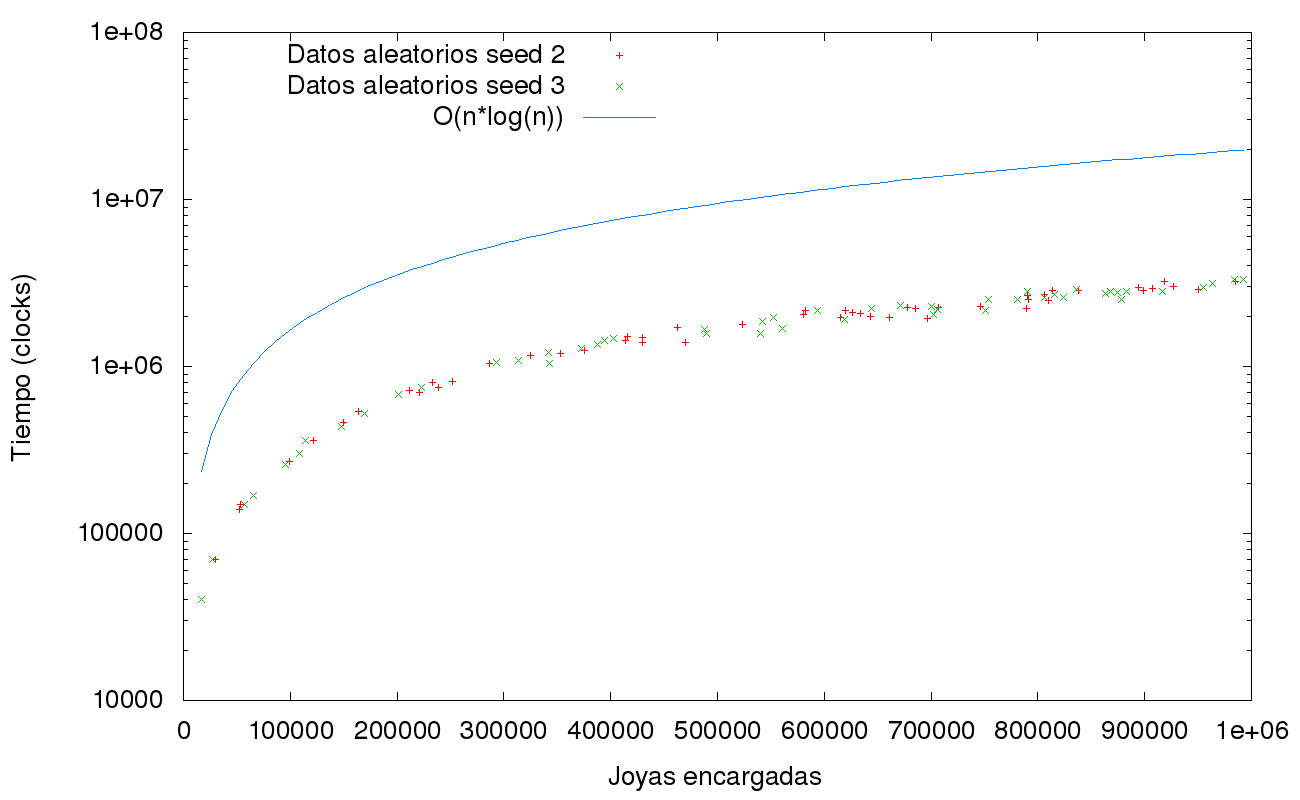
\includegraphics[scale=0.4]{./img/ej2_chart2.png}
\caption{Tiempo transcurrido por encargos de joyas}
\end{figure}
\end{center}

Como se puede observar el algoritmo corre en tiempos de ejecuci\'on bastante inferiores a la cota m\'axima propuesta de $O(n*log(n))$, a partir de un $n_{0}$
